\documentclass{article}

\usepackage[margin = 1in]{geometry}
\usepackage{graphicx, amsmath}
\graphicspath{ {./images/} }

\title{Ch. 5 Solutions}
\author{Principles of Microeconomics}
\date{\today}

\begin{document}

\maketitle

\section*{Quick Quiz}

\begin{enumerate}

\item (a) -- If a good is a necessity, that means there aren't many if any substitutes. Therefore consumers can't reduce their demand much in response to a price increase. 

\item (d) -- An increase in price leads to a decrease in total revenue if demand is elastic.

\item (d) -- The elasticity of a linear demand curve is non-constant.

\item (c) -- If the income elasticity of demand is 0.5, the decrease in income between Gondor and Rohan leads to a proportionately smaller decrease in $Q_D$. Since Rohan's income declines more than its quantity demanded relative to Gondor, Rohan must spend a higher fraction of its income on food. 

\item (b) --
	\begin{gather*}
	\% \Delta P = \frac{24 - 16}{\frac{24 + 16}{2}} = \frac{8}{20} = \frac{2}{5} \\
	\% \Delta Q = \frac{110 - 90}{\frac{110 + 90}{2}} =  \frac{20}{100} = \frac{1}{5} \\
	\text{Price Elasticity of Supply} = \frac{\% \Delta Q}{\% \Delta P} = \frac{1}{2} = 0.5.
	\end{gather*}
	
\item (c) -- If the price elasticity of supply is zero, that means the supply curve is perfectly inelastic, and perfectly inelastic supply is vertical.

\item (c) -- The ability of firms to enter and exit a market in the long run gives sellers more flexibility to change the amount they produce, so it makes the supply curve more elastic.

\item (c) -- If the demand curve is inelastic, an increase in supply will decrease price proportionately more than it will increase quantity. As a result, revenue will go down.

	\begin{center}
	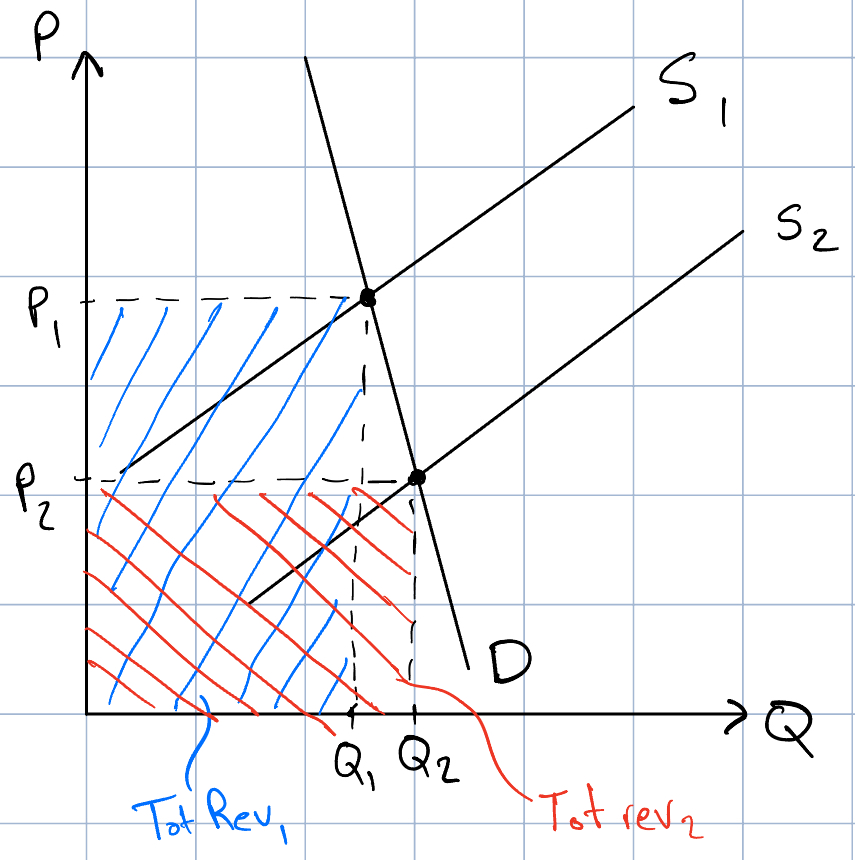
\includegraphics[width = 0.3\textwidth]{ch5_qq8}
	\end{center}
	
\item (a) -- Since each farmer takes the market price as given, they must choose between producing more or producing less at that price. They will always choose to produce more because producing less lowers their revenue and therefore their income.

\item (c) -- When supply shifts left by a given amount, the change in the equilibrium price depends on the elasticity of the demand curve. The more elastic demand is, the less price will increase. In the long run, demand for oil is more elastic, so OPEC's supply reduction caused less of a price increase. See Figure 8.

\item (b) -- For quantity demanded to go up when incomes go up, smartphones must be a normal good. That means the income elasticity of demand must be greater than 0. For total expenditure (a.k.a. revenue) to increase when price decreases, quantity demanded must increase proportionately more than price decreases. That means the numerator of the price elasticity of demand equation must be bigger than the denominator, so the price elasticity of demand must be greater than one. 

\end{enumerate}

\section*{Questions for Review}

\begin{enumerate}

\item The price elasticity of demand is: \[ \left| \frac{\% \Delta Q_D}{\% \Delta P} \right|. \] It measures how responsive the quantity demanded of a good is to a change in price.

The income elasticity of demand is: \[ \frac{\% \Delta Q_D}{\% \Delta I} \] where $I$ is income. It measures how responsive the quantity demanded of a good is to a change in buyers' income.

\item
	\begin{itemize}
	
	\item Substitutability -- The more substitutes a good has, the more responsive people will be to a change in price. Therefore, goods with more substitutes have more elastic demand.
	
	\item Necessity v. Luxury -- Necessities have less elastic demand while luxuries have more elastic demand. That's because true necessities have few substitutes while luxuries have many substitutes. 
	
	\item Market Breadth -- The more narrowly defined a market is, the more elastic its demand. That's because it's easier to find substitutes for narrowly defined markets. For example, clothing -- a broad market -- will have less elastic demand than henley t-shirts -- a narrow market. 
	
	\item Time Horizon -- Over the long term, demand for most goods is more elastic. That's because it is easier for people to find substitutes given more time. 
	
	\end{itemize}
	
\item If the elasticity is greater than one, a one percent change in price causes a greater than one percent change in quantity demanded. That means quantity demanded is highly responsive to a change in price, so demand is elastic.

If the elasticity equals zero, then a one percent change in price causes a zero percent change in quantity demanded. That means quantity demanded is completely unresponsive to a change in price, so demand is perfectly inelastic.

\item \phantom{x}
	\begin{center}
	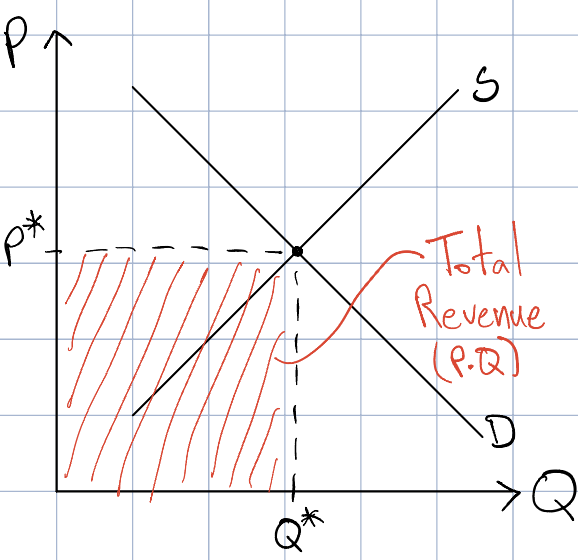
\includegraphics[width = 0.3\textwidth]{ch5_qfr3}
	\end{center}
	
\item If demand is elastic, an increase in the price will cause a proportionately greater decrease in the quantity demanded. Therefore, total revenue, $P \cdot Q$, will decrease because $Q$ decreases more than $P$ increases.

\item If income elasticity is less than zero, then a positive change in income causes a negative change in quantity demanded. In other words, an increase in income causes a decrease in quantity demanded. That's true for inferior goods.

\item The price elasticity of supply is: \[ \frac{\% \Delta Q_S}{\% \Delta P}. \] To calculate the percent changes, we use the midpoint method: \[ \frac{X_f - X_i}{\left(\frac{X_f + X_i}{2}\right)}. \]

The price elasticity of supply measures how responsive the quantity supplied of a good is to a change in price. 

\item If a fixed quantity is available regardless of the price, then the price elasticity of supply is zero. That means that the quantity supplied is completely unresponsive to a change in price.

\item If demand is very elastic, the drop in supply will decrease quantity by more than it will increase price. As a result, total revenue will fall. Conversely, if demand is very inelastic, the drop in supply will decrease quantity by less than it will increase price. As a result, total revenue will increase. Therefore, the event is more likely to hurt fava bean farmers if the demand for fava beans is very elastic. 
	\begin{center}
	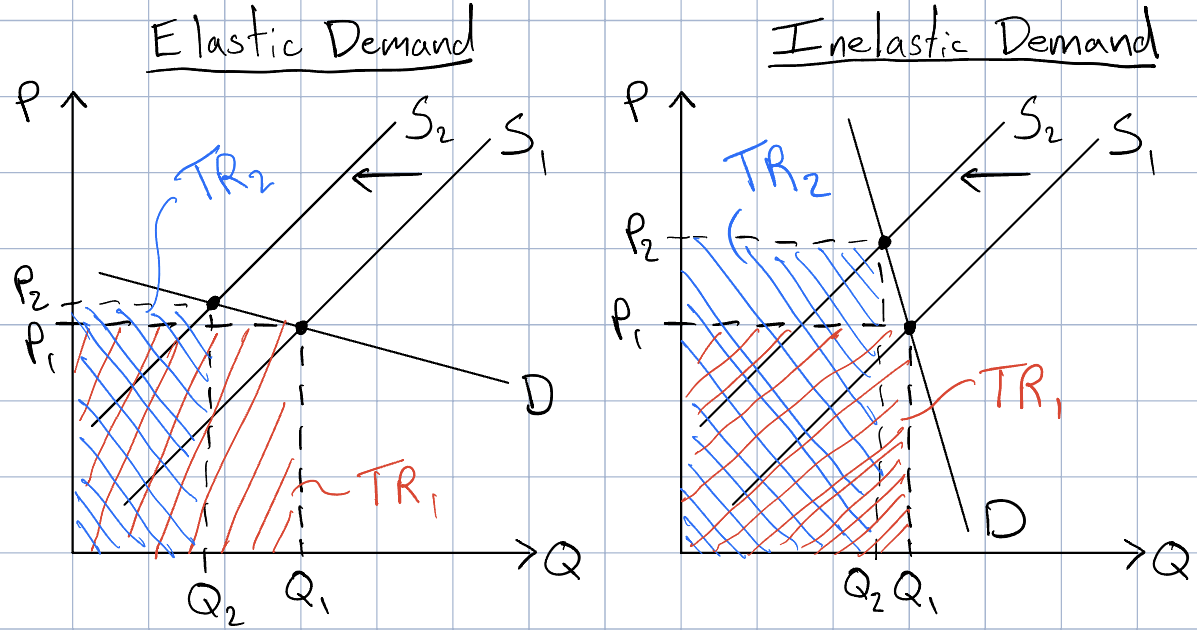
\includegraphics[width = 0.6\textwidth]{ch5_qfr9}
	\end{center}

\end{enumerate}

\section*{Problems and Applications}

\begin{enumerate}

\item

	\begin{enumerate}
	
	\item I'd expect mystery novels to be more elastic because they're more substitutable than a required textbook.
	
	\item I'd expect Billie Eilish recordings to be more elastic because they are a more narrowly defined good.
	
	\item I'd expect subway rides during the next five years to be more elastic because the longer time horizon gives people more time to change their behavior and find substitutes.
	
	\item I'd expect root beer to be more elastic because it is more of a luxury than water. 
	
	\end{enumerate}
	
\item
	
	\begin{enumerate}
	
	\item 
	
		\begin{enumerate}
		
		\item 
		\begin{gather*}
		\% \Delta Q = \frac{1900 - 2000}{\frac{1900 + 2000}{2}} = \frac{-100}{1950} = -\frac{2}{39} \\
		\% \Delta P = \frac{250 - 200}{\frac{250 + 200}{2}}  = \frac{50}{225} = \frac{2}{9} \\
		\eta = \left| \frac{\% \Delta Q}{\% \Delta P} \right| = \frac{\frac{2}{39}}{\frac{2}{9}} = \frac{9}{39} \approx 0.23
		\end{gather*}
		
		\item
		\begin{gather*}
		\% \Delta Q = \frac{600 - 800}{\frac{600 + 800}{2}} = \frac{-200}{700} = \frac{-2}{7} \\
		\% \Delta P = \frac{2}{9} \text{ (See above)} \\
		\eta = \left| \frac{\% \Delta Q}{\% \Delta P} \right| = \frac{\frac{2}{7}}{\frac{2}{9}} = \frac{9}{7} \approx 1.29
		\end{gather*}
		
		\end{enumerate}
		
	\item Flights are more of a necessity for business travelers and more of a luxury for vacationers, so we would expect vacationers to have more elastic demand.
	
	\end{enumerate}
	
\item

	\begin{enumerate}
	
	\item Short run:
	\begin{align*}
	\% \Delta P &= \frac{2.2 - 1.8}{\frac{2.2 + 1.8}{2}} = \frac{0.4}{2} = 0.2\% \\
	\eta_D &= \left| \frac{\% \Delta Q_D}{\% \Delta P} \right| \\
	0.2 &= \frac{| \% \Delta Q_D |}{0.2} \\
	0.04\% &= | \% \Delta Q_D | \\
	-0.04\% &= \% \Delta Q_D \text{ (by the law of demand)}
	\end{align*}
	
	Long run:
	\begin{align*}
	\eta_D &= \left| \frac{\% \Delta Q_D}{\% \Delta P} \right| \\
	0.7 &= \frac{| \% \Delta Q_D |}{0.2} \\
	0.14\% &= | \% \Delta Q_D | \\
	-0.14\% &= \% \Delta Q_D \text{ (by the law of demand)}
	\end{align*}
	
	\item A longer time horizon gives people more time to find substitutes for heating oil and change their behavior. For example, they could switch their home to natural gas. Therefore, we expect elasticity to increase over the long run.
	
	\end{enumerate}
	
\item If total revenue increases, price must increase proportionately more than quantity demanded decreases. That means the change in $Q_D$ is smaller than the change in $P$, so the elasticity is less than one. Therefore, demand is inelastic.

\item

	\begin{enumerate}
	
	\item The hurricane decreases the supply of coffee beans, so supply shifts left. As a result, price increases.
	
	\begin{center}
	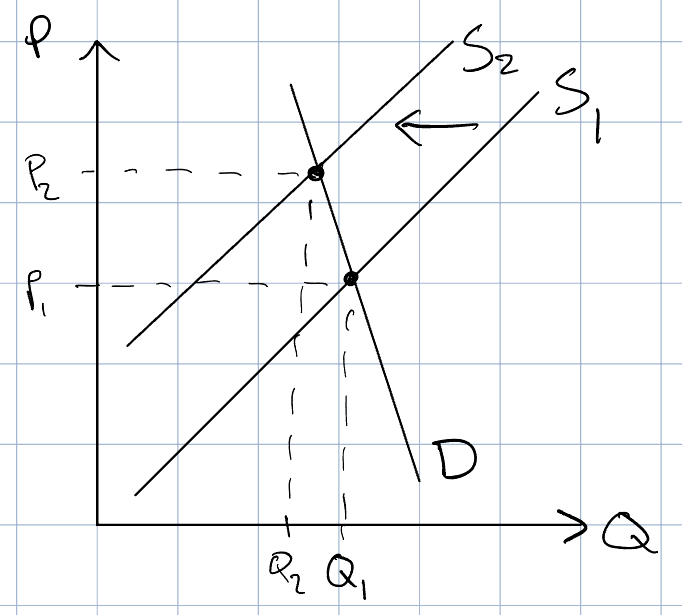
\includegraphics[width = 0.3\textwidth]{ch5_paa5a}
	\end{center}
	
	\item Because the price of coffee beans, an input, increased, the supply of cups shifts left. As a result price increases, and quantity decreases. Since demand is inelastic, the increase in price is proportionately larger than the decrease in quantity. That means total expenditure increases.
	
	\begin{center}
	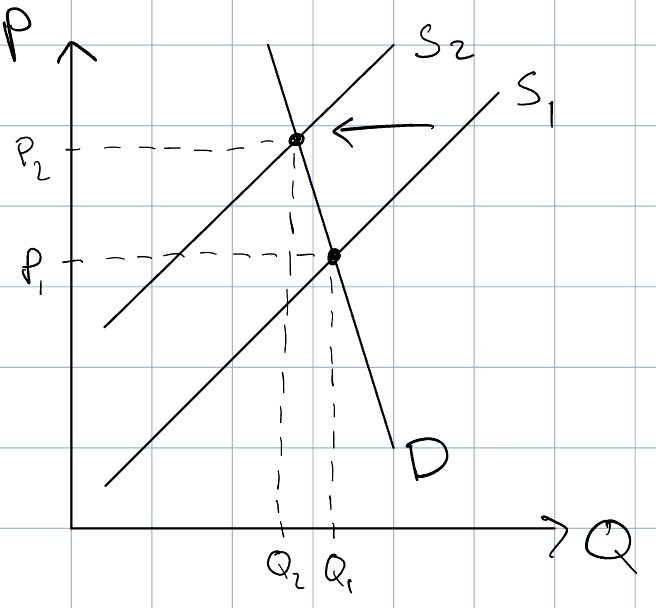
\includegraphics[width = 0.3\textwidth]{ch5_paa5b}
	\end{center}
	
	\newpage
	
	\item The price of a complement went up, so demand for donuts decreases. Therefore, quantity and price both decrease which means total expenditure decreases as well.
	
	\begin{center}
	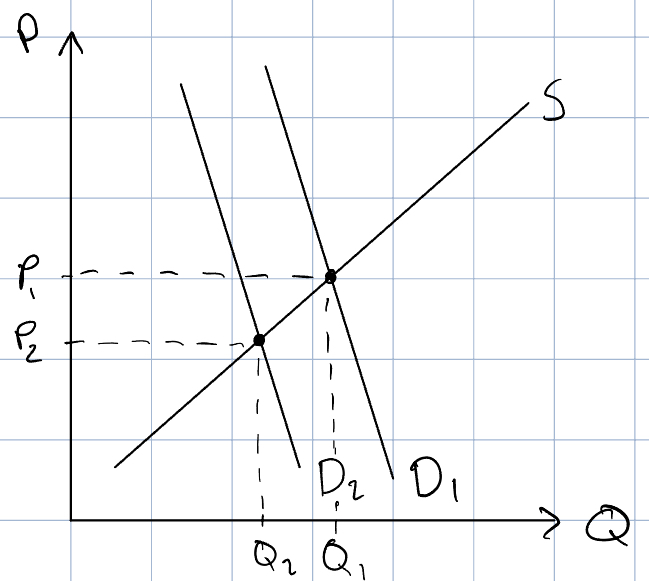
\includegraphics[width = 0.3\textwidth]{ch5_paa5c}
	\end{center}
	
	\end{enumerate}
	
\item Meredith, Miranda, and Owen could all be right. For Miranda to be right, the curves would have to shift in such a way that the equilibrium quantity didn't change.
	\begin{center}
	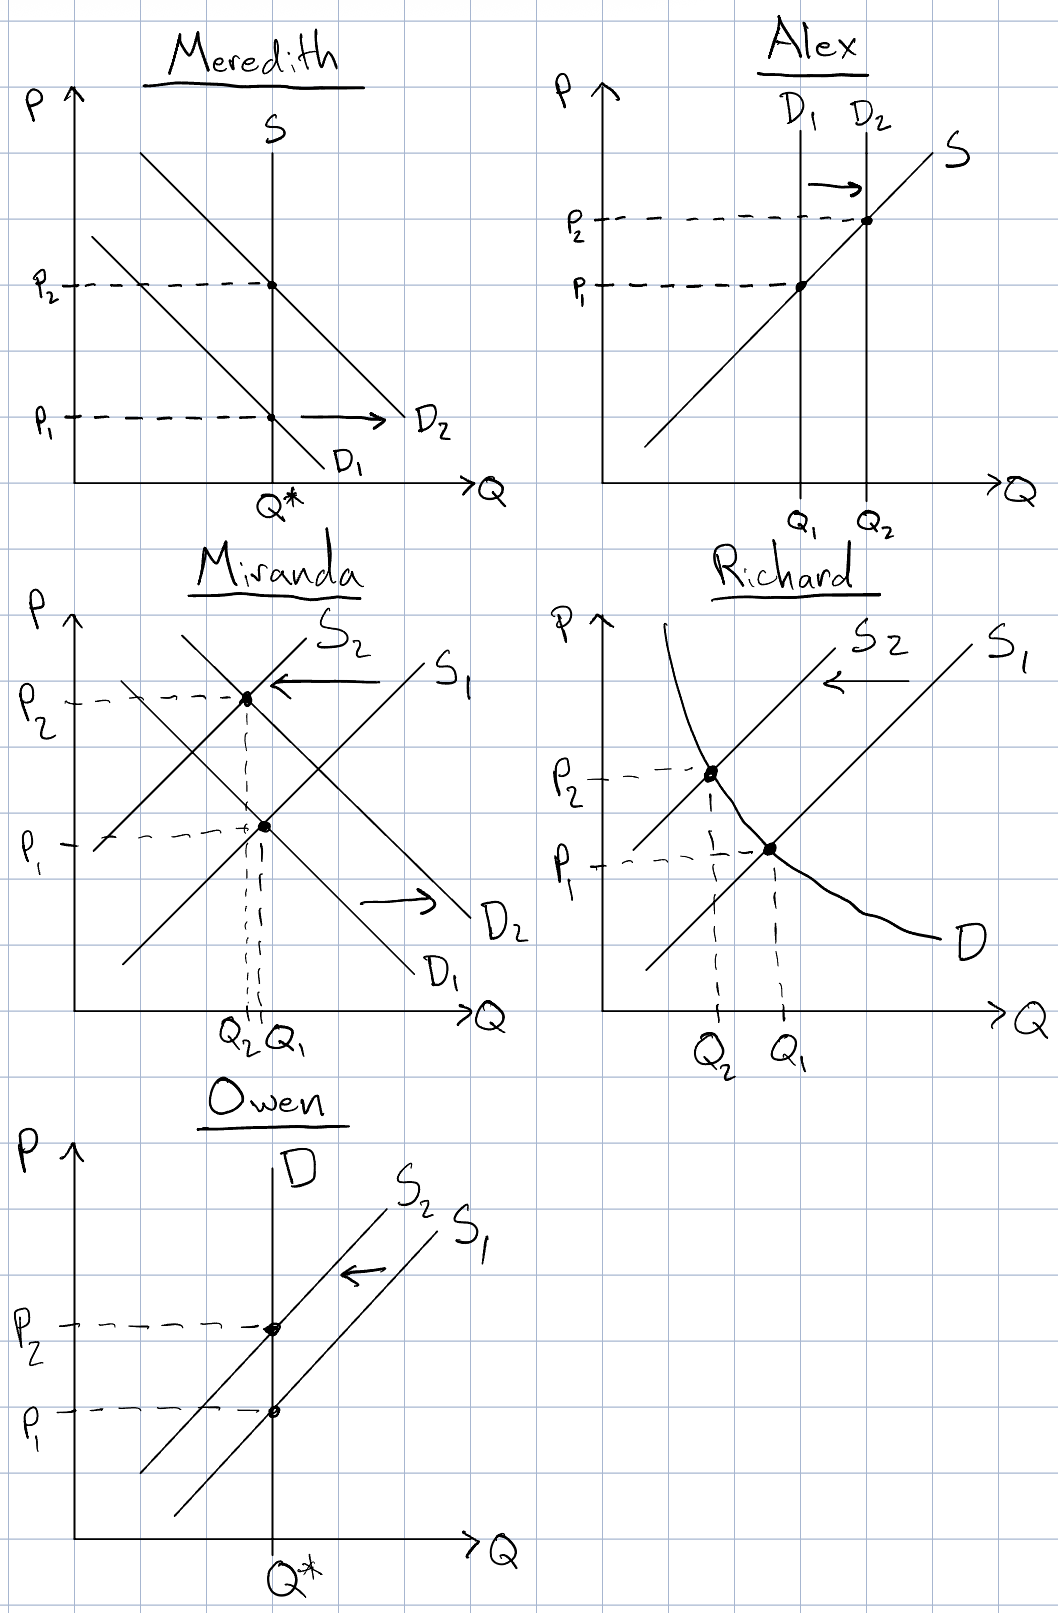
\includegraphics[width = 0.6\textwidth]{ch5_paa6}
	\end{center}
	
\item

	\begin{enumerate}
	
	\item
	
		\begin{enumerate}
		
		\item 
		\begin{gather*}
		\% \Delta Q = \frac{32 - 40}{\frac{32 + 40}{2}} = -\frac{8}{36} = -\frac{2}{9} \\
		\% \Delta P = \frac{10 - 8}{\frac{10 + 8}{2}} = \frac{2}{9} \\
		\eta = \left| \frac{\% \Delta Q}{\% \Delta P} \right| = 1
		\end{gather*}
		
		\item
		\begin{gather*}
		\% \Delta Q = \frac{45 - 50}{\frac{45 + 50}{2}} = \frac{-5}{47.5} = -\frac{10}{95} \\
		\% \Delta P = \frac{2}{9} \\
		\eta = \left| \frac{\% \Delta Q}{\% \Delta P} \right| = \frac{90}{190} = \frac{9}{19} \approx 0.47
		\end{gather*}
		
		\end{enumerate}
	
	\item
	
		\begin{enumerate}
		
		\item
		\begin{gather*}
		\% \Delta Q = \frac{30 - 24}{\frac{30 + 24}{2}} = \frac{6}{27} = \frac{2}{9} \\
		\% \Delta I = \frac{24,000 - 20,000}{\frac{24,000 + 20,000}{2}} = \frac{4,000}{22,000} = \frac{2}{11} \\
		IED = \frac{\% \Delta Q}{\% \Delta I} = \frac{\frac{2}{9}}{\frac{2}{11}} = \frac{11}{9} \approx 1.22
		\end{gather*}
		
		\item
		\begin{gather*}
		\% \Delta Q = \frac{12 - 8}{\frac{12 + 8}{2}} = \frac{4}{10} = \frac{2}{5} \\
		\% \Delta I = \frac{2}{11} \\
		IED = \frac{\% \Delta Q}{\% \Delta I} = \frac{\frac{2}{5}}{\frac{2}{11}} = \frac{11}{5} = 2.2
		\end{gather*}
		
		\end{enumerate}
	
	\end{enumerate}

\item

	\begin{enumerate}
	
	\item 
	
		\begin{gather*}
		\% \Delta Q = -0.043 \\
		\% \Delta P = \frac{1.5 - 1.25}{\frac{1.5 + 1.25}{2}} = \frac{0.25}{1.375} \approx 0.18 \\
		\eta = \left| \frac{\% \Delta Q}{\% \Delta P} \right| \approx 0.24
		\end{gather*}
		
	\item Based on my estimate, demand for subway rides is inelastic. Therefore, when the Transit Authority raises fares, we should expect revenue to increase. That's because quantity demanded will decrease proportionately less than fares will increase. 
	
	\item The estimate is unreliable because there could be other reasons for the decrease in ridership. For example, it's possible that gas was cheaper and the weather was worse in December 1995. If that were the case, people would be more inclined to drive or stay home than they would be to take the subway. (This question doesn't test anything we've learned. It's just a common sense question that hints at econometrics, a statistics course you'll take in college if you choose to pursue economics.) 
	
	\end{enumerate} 
	
\item Thelma's demand is perfectly inelastic ($\eta = 0$) because she demands the same quantity regardless of price. Louise's demand is unit elastic ($\eta = 1$) because her total expenditure (price times quantity) is constant at \$20 regardless of the price. For her total expenditure to be constant, any change in the price must be offset by a change in her quantity demanded. That's only true if her demand is unit elastic.

\item

	\begin{enumerate}
	
	\item 
	
		\begin{gather*}
		\eta = \left| \frac{\% \Delta Q}{\% \Delta P} \right| \\
		0.4 = \left| \frac{-20 \%}{\% \Delta P} \right| \\
		\% \Delta P = \frac{20}{0.4} \\
		\% \Delta P = 50 \\
		100 * \frac{P_2 - 5}{\frac{P_2 + 5}{2}} = 50 \\
		P_2 - 5 = 0.25P_2 + 1.25 \\
		0.75P_2 = 6.25 \\
		P_2 \approx \$8.33
		\end{gather*}
		
		The government should increase the price by 50\%. If you use the midpoint method, that's an increase of \$3.33. If you don't use the midpoint method, that's an increase of \$2.50.
		
	\item The policy will have a larger effect five years from now. In the long run, demand will be more elastic, so quantity demanded will decrease more in response to the price increase. 
	
	\item Teenager smokers might have developed less of a nicotine addiction than adult smokers. As a result, they might treat cigarettes as more of a luxury good while adult smokers might treat them as more of a necessity.
	
	\end{enumerate}
	
\item It depends on the price elasticity of demand for museum admission. If demand is elastic, the museum should decrease the price of admission. That's because the quantity of tickets demanded will increase proportionately more than price will decrease. When quantity increases more than price decreases, revenue increases.

If demand is inelastic, the museum should increase the price of admission. That's because the quantity of tickets demanded will decrease proportionately less than price will increase. When quantity decreases less than price increases, revenue increases.

I imagine demand for museum admission is elastic because it's a highly substitutable activity.

\item Demand for grains from around the world is inelastic because grains are a staple food with few good substitutes. When a drought hits around the world, the global grain supply shifts left driving price up and quantity down. Since demand is inelastic, the increase in price is proportionately larger than the decrease in quantity, so total revenue increases.

Demand for grains from Kansas is elastic because there are lots of substitutes -- grains from anywhere else in the world. When a drought hits Kansas, the supply of grains from Kansas shifts left driving price up and quantity down. Since demand is elastic, the decrease in quantity is proportionately larger than the increase in price, so total revenue falls.

******************************** Need to add graphs **************************************

\end{enumerate}

\section*{Non-Textbook Questions}

\begin{enumerate}

\item

	\begin{enumerate}
	
	\item Increase -- the introduction of alternative SUVs will increase the substitutability of Ford SUVs.
	
	\item Decrease -- the removal of alternative SUVs will decrease the substitutability of Ford SUVs.
	
	\item Decrease -- if people think that SUVs are uniquely safe, that will decrease their substitutability. 
	
	\item Increase -- a longer time horizon gives buyers more time to find substitutes and sellers more time to offer substitutes.
	
	\end{enumerate}
	
\item

	\begin{enumerate}
	
	\item
		\begin{gather*}
		PES = \frac{\% \Delta Q_S}{\% \Delta P} \\
		1.6 = \frac{\% \Delta Q_S}{-0.18} \\
		-0.288 = \% \Delta Q_S
		\end{gather*}
		$Q_S$ decreases by 28.8\%.
		
	\item
		\begin{gather*}
		IED = \frac{\% \Delta Q_D}{\% \Delta I} \\
		0.6 = \frac{\% \Delta Q_D}{ \frac{42,000 - 38,000}{40,000} } \\
		0.6 = \frac{\% \Delta Q_D}{0.1} \\
		0.06 = \% \Delta Q_D
		\end{gather*}
		$Q_D$ increases by 6\%.
		
	\item The cross-price elasticity of demand would be negative because the two goods are complements. An increase in the price of iPhones will decrease the quantity demanded of portable chargers.
	
	\item Let $x = \% \Delta Q_D$.
		\begin{gather*}
		TR = PQ \\
		1.02TR = 1.05P*(1 + x)Q \\
		1.02TR = 1.05(1 + x) PQ \\
		1.02 = 1.05(1 + x) \\
		\frac{1.02}{1.05} - 1 = x \\
		-0.03 \approx x
		\\
		\eta \approx \left| \frac{-3\%}{5\%} \right| = 0.6
		\end{gather*}
	
	\end{enumerate}
	
\item The technological breakthrough causes supply to shift right. As a result, price decreases and quantity increases. For total revenue to go up, the increase in quantity must be proportionately larger than the decrease in price. That will be true if demand is elastic.
	\begin{center}
	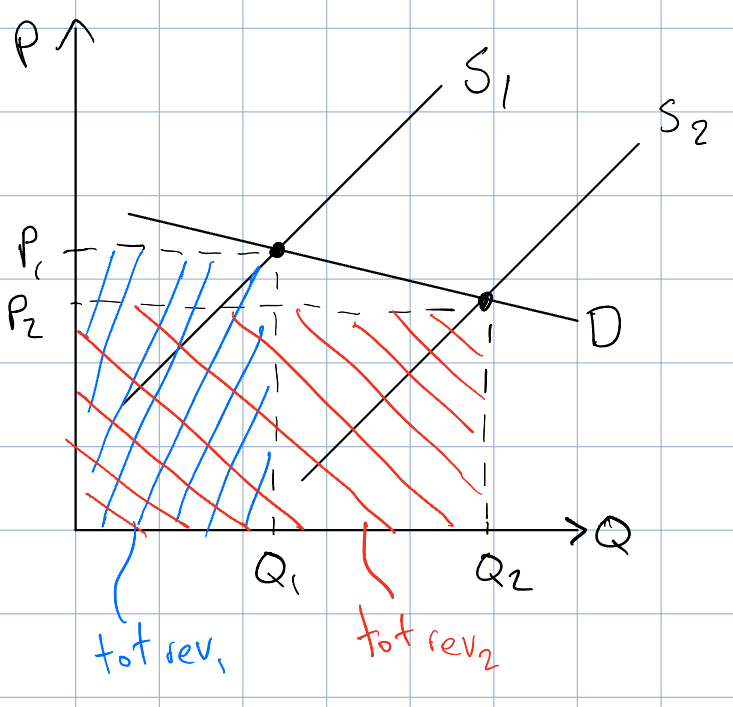
\includegraphics[width = 0.3\textwidth]{ch5_ntq4}
	\end{center}
	
\item Let $x = \% \Delta Q_D$.
	\begin{gather*}
	1.05PQ = 1.1P*(1 + x)Q \\
	1.05PQ = 1.1(1+x)PQ \\
	1.05 = 1.1(1+x) \\
	\frac{1.05}{1.1}-1 = x \\
	-0.05 \approx x
	\end{gather*}
	$Q_D$ decreased by 5\%.
	\begin{gather*}
	\eta \approx \left| \frac{-0.05}{0.10} \right| \\
	\eta \approx 0.5
	\end{gather*}
	Demand is inelastic because $\eta \approx 0.5$.
	
	Alternatively, this problem doesn't explicitly ask you to calculate $\eta$, so you could infer that demand is inelastic from the fact that an increase in price raised revenue. That means the change in price was proportionately larger than the change in quantity demanded. That implies that demand is inelastic.
	
	Taxicab drivers were assuming that demand was perfectly inelastic. For a 10\% increase in price to cause a 10\% increase in revenue, the quantity demanded would have to remain constant despite the change in price.


\end{enumerate}

\end{document}